\chapter{Laplace Transforms}
\chapter*{Lecture 27}

\begin{recall}{}{}
\begin{itemize}
\item Next Monday/Tuesday: no MTE202 (instead 2h on Wed 21/28 Nov), 
 \item Course evaluation by Friday
\item Completed chapter on linear-second order equations
\end{itemize}
\end{recall}


\section{Introduction}
\begin{itemize}
\item Recall a typical constant coefficient, non-homogeneous 2nd order ODE:
\begin{equation*}
y''+5y'+6y=3x^2
\end{equation*}
This equation can be solved via MUC because our forcing term is continuous.
\item What if the forcing term is discontinuous?

\begin{equation*}
y''+5y'+6y=
\begin{cases}
    3x^2,& \text{if } 0\leq x< 1\\
    1,   &  \text{if } x> 1
\end{cases}
\end{equation*}
with $y(0)=y_0$ and $y'(0)=V_0$. Here the forcing term is a discontinuous function.

If we try to solve using standard approaches from chapter 4, we :
\begin{itemize}
\item first solve:
\begin{equation*}
y''+5y'+6y=3x^2
\end{equation*}
with initial conditions $y(0)=y_0$ and $y'(0)=V_0$ for $0\leq x<1$
\item Then solve:
\begin{equation*}
y''+5y'+6y=1
\end{equation*}
with initial conditions $y(1)=y_1$ and $y'(1)=V_1$ (from previous solution) for $x>1$
\end{itemize}

\item What if we have alternating current?

\begin{figure}
\centering
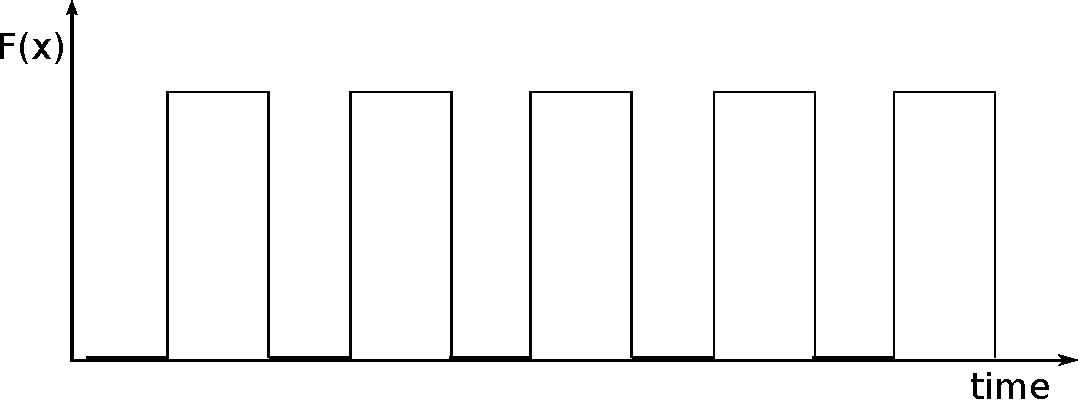
\includegraphics[width=0.8\textwidth]{figs/AC_current.pdf} 
\caption{Alternating current example.}
\end{figure}
If we solved the following example using the classical approaches, we would need to solve MANY ODES!

Is there a better choice to solve these equations? Laplace transform method (L.T.)\\
\end{itemize}
\textbf{Laplace transforms are one of the most IMPORTANT concepts in engineering mathematics, especially control theory.}


\subsection{Laplace transforms}

A Laplace transform, changes the solution from a time-domain to an $s$-domain:
\begin{equation*}
\Lapl\left(f(t) \right) \rightarrow F(s)
\end{equation*}
What is a transform?
\begin{itemize}
\item A function takes from one set of numbers to another set numbers.
\item A transforms takes from one set of functions to another set of functions!
\end{itemize}

For a given function $f(t)$, its Laplace transform is:
\begin{equation}
\boxed{F(s)=\Lapl\left( f(t) \right) =\int^\infty_0 e^{-st} f(t) dt}
\end{equation}
where $F(s)$ is the transformed function in the $s$-domain, $\Lapl$ the Laplace transform operator, $e^{-st}$ the kernel of the operator and $f(t)$ the function in time domain.



\subsection*{Merits of Laplace transforms}
\begin{itemize}
\item Transforms discontinuous functions into a single continuous function
\item Transforms differential equations into algebraic equations
\item Incorporates the initial condition directly into the algebraic equations (no need to apply ICs)
\end{itemize}





\begin{exmp}{LT:}\\
Find the LT of $f(t)=e^{\alpha t}$.\\
\textbf{Solution:}
\begin{align*}
\Lapl\left( f(t) \right) &=\int^\infty_0 e^{-st} e^{\alpha t} dt\\
  & =\int^\infty_0 e^{-(s-\alpha)t}  dt\\
    & =\left. \frac{1}{-(s-\alpha)}e^{-(s-\alpha)t}  \right|^\infty_0\\
    & =\lim_{t\to\infty}\left[\frac{-1}{s-\alpha}\frac{1}{e^{(s-\alpha)t}}\right]+\frac{1}{s-\alpha}
\end{align*}
Three cases are possible
\begin{itemize}
\item $s>\alpha$ therefore $s-\alpha>0$: $\lim_{t\to\infty}\frac{1}{e^{(s-\alpha)t}}$. Thus:
\begin{equation*}
F(s)=\frac{1}{s-\alpha}
\end{equation*}
\item  $s<\alpha$ therefore $s-\alpha<0$: $\lim_{t\to\infty}\frac{1}{e^{(s-\alpha)t}} \infty $. Thus:
\begin{equation*}
F(s)=\infty \qquad \qquad \text{diverged!}
\end{equation*}
\item  $s=\alpha$ therefore $s-\alpha=0$. Thus:
\begin{align*}
\Lapl\left( f(t) \right)  =\int^\infty_0 e^{-st} e^{\alpha t} dt=\int^\infty_0 dt \left. t\right|^\infty_0=\infty
\end{align*}
\end{itemize}
$\Lapl\left( f(t) \right) $ exists only when $s>\alpha$:
\begin{align*}
\boxed{\Lapl\left(  e^{\alpha t} \right) =\frac{1}{s-\alpha}}
\end{align*}
\end{exmp}



\begin{exmp}{LT:}\\
Find the LT of $f(t)=t$.\\
\textbf{Solution:}
\begin{align*}
\Lapl\left( f(t) \right) &=\int^\infty_0 e^{-st} t dt\\
\end{align*}
Integration by parts:
\begin{align*}
u &=t \qquad \qquad & v=\frac{-e^{-st}}{s}\\
du&=dt & dv=e^{-st} dt
\end{align*}
(assume $s>0$)
\begin{align*}
\Lapl\left( f(t) \right) &=\left[uv-\int v du\right]^\infty_0\\
&=\left[\frac{-e^{-st} t}{s}\right]^\infty_0+\frac{1}{s}\int^\infty_0 e^{-st}dt
&=0-\left.\frac{1}{s^2}e^{-st}\right|^\infty_0
\end{align*}
\begin{align*}
\boxed{ \Lapl(t) =\frac{1}{s^2}}
\end{align*}
\end{exmp}
